\documentclass[10pt]{beamer}

% Escolha do tema
\usetheme{Ilmenau}

% Estes 3 são básicos para português com acentuação correta no PDF:
\usepackage[utf8]{inputenc}   % (Pode ser removido em distribuições TeX mais recentes, que já assumem UTF-8.)
\usepackage[T1]{fontenc}
\usepackage[brazil]{babel}
\usepackage{bookmark}
\usepackage{hyperref}
% Se quiser inserir figuras futuramente, mantenha:
%\usepackage{graphicx} % Se quiser inserir figuras futuramente, mantenha.
%\usepackage{amsmath, amssymb, amsfonts} % Se não tiver fórmulas avançadas, pode dispensar os pacotes de matemática.
%\usepackage{mathtools} % Se não tiver fórmulas avançadas, pode dispensar os pacotes de matemática.
%\usepackage{multirow} % Se não usa mais de uma linha numa mesma célula de tabela, pode remover.
%\usepackage{comment} % Se não tem blocos de texto enormes para comentar, pode remover.
%\usepackage{colortbl} % Se não usa coloração manual de tabelas, pode remover.
%\usepackage{ulem} % Se não precisa riscar texto com \sout, pode remover.
%\usepackage{ragged2e} % Se não usa alinhamentos especiais (por exemplo, \justifying), pode remover.
%\usepackage{array} % Se não tem tabelas avançadas ou arranjos especiais, pode remover.
%\usepackage{tikz} % Se não desenha nada com TikZ, pode remover.
%\usetikzlibrary{positioning, matrix, chains, decorations.pathreplacing, arrows} % Se não desenha nada com TikZ, pode remover.
%\usepackage{algorithm, algpseudocode} % Se não apresenta algoritmos, pode remover.
%\usepackage{animate} % Se não faz animações, pode remover.
%\usepackage{caption} % Se não vai usar legendas customizadas ou subfiguras, pode remover.
%\usepackage{subcaption} % Se não vai usar legendas customizadas ou subfiguras, pode remover.
%\usepackage{verbatim} % Se não precisa de ambientes verbatim especiais (texto literal), pode remover.

% Ajuste de margens no Beamer (em vez de geometry)
\setbeamersize{text margin left=0.5cm, text margin right=0.5cm}

% Definição do título
\title[Reunião de Acompanhamento no CTMRJ (MAR2025)]{Reunião de Acompanhamento do Mestrado}


\title{\textbf{Proposta de Projeto:} Planejamento Dinâmico de Rotas para VANTs em Patrulha Naval}

\author[UFRJ / COPPE / PESC / CPS767 -- \textit{Algoritmos de Monte Carlo e Cadeias de Markov}]{
  \textbf{Aluno:} Luiz Henrique Souza Caldas -- \texttt{lhscaldas@cos.ufrj.br} \newline
  \textbf{Prof.:} Daniel Ratton Figueiredo
}

\institute[]{UFRJ / COPPE / PESC \newline
CPS767 -- \textit{Algoritmos de Monte Carlo e Cadeias de Markov}}
\date{\today}

\begin{document}

\frame{\titlepage}

\begin{frame}{Motivação}
    \begin{columns}
        \column{0.5\textwidth}
        \centering
        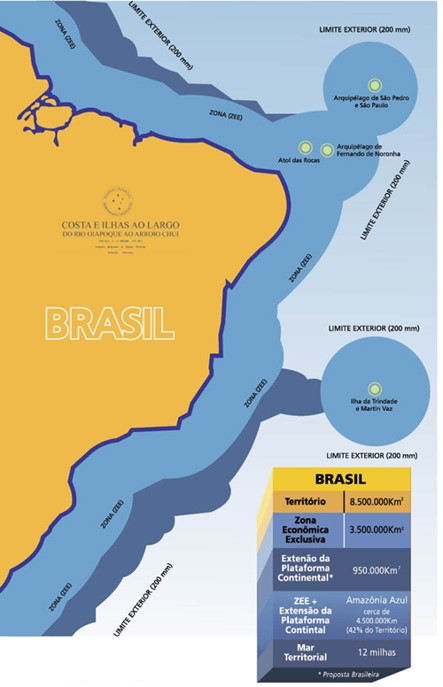
\includegraphics[width=0.8\linewidth]{fig/amazonia_azul.jpg}
        \column{0.5\textwidth}
        \centering
        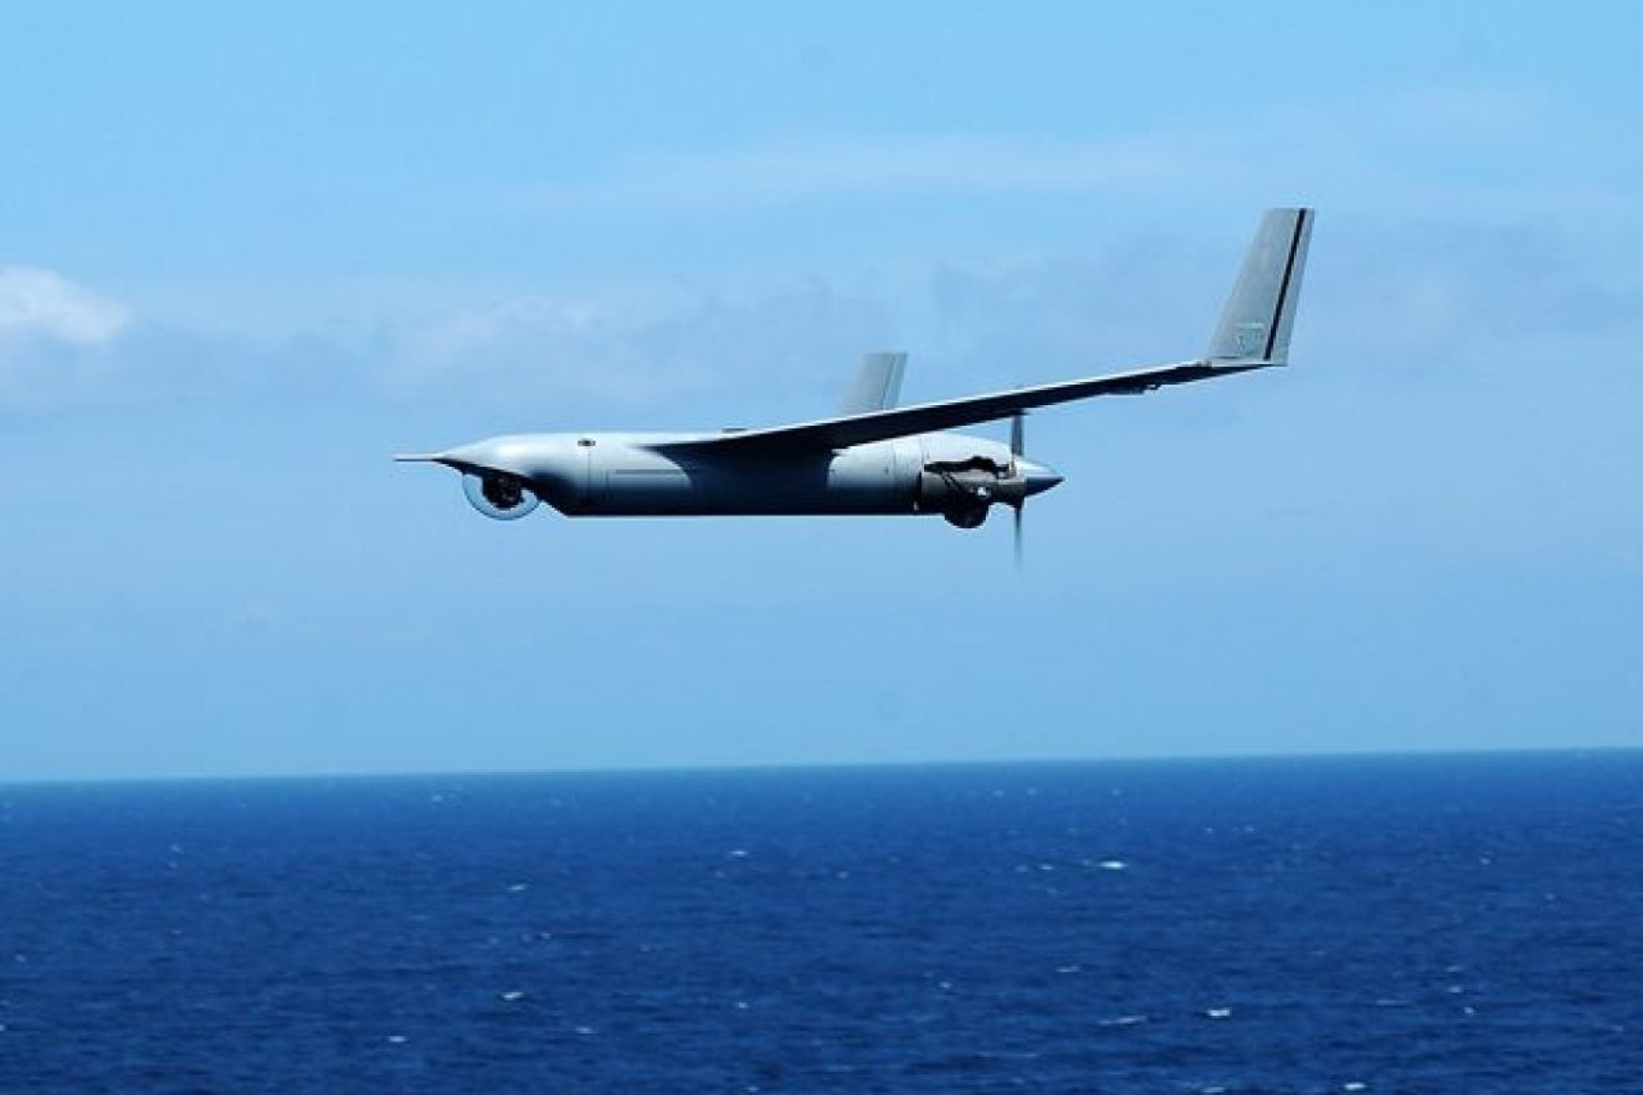
\includegraphics[width=0.8\linewidth]{fig/scan_eagle.jpg}
        \begin{itemize}
            \item 4,5 milhões de km² de área marítima
            \item Necessidade de patrulha naval eficiente
            \item Uso de VANTs para reconhecimento e vigilância
        \end{itemize}
    \end{columns}
\end{frame}

\begin{frame}{Problema}
    \begin{columns}
        \column{0.5\textwidth}
        \centering
        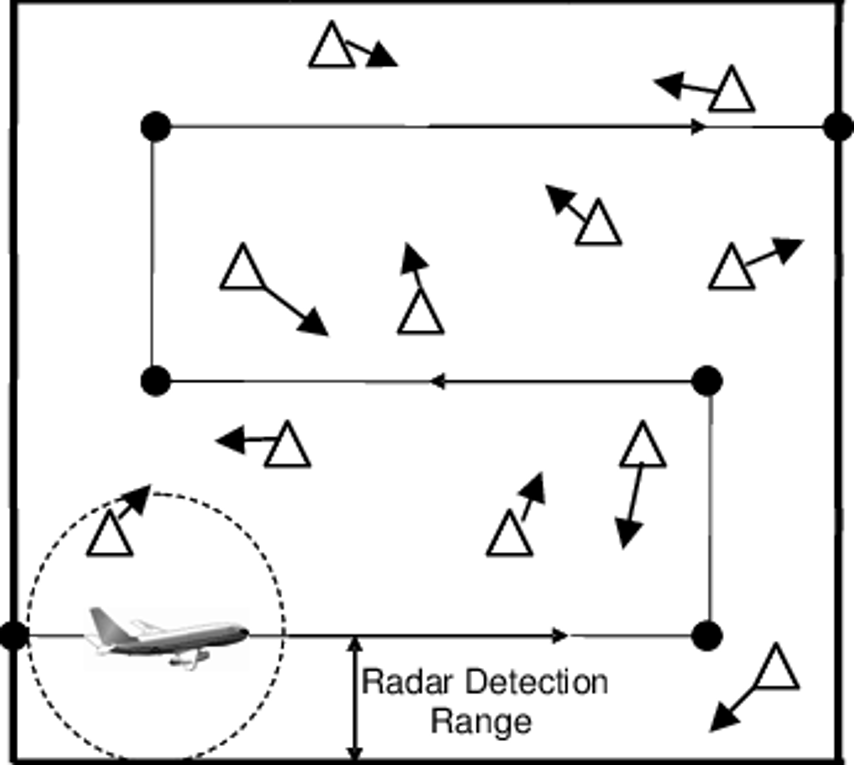
\includegraphics[width=\linewidth]{fig/vant.png}
        \column{0.5\textwidth}
        \centering
        \begin{itemize}
            \item Alcance do radar vs. câmera
            \item Alvos surgem dinamicamente durante a missão
            \item Autonomia limitada (combustível)
            \item Objetivo: maximizar o número de alvos inspecionados
        \end{itemize}
    \end{columns}
\end{frame}

\begin{frame}{Metodologia}
    \begin{columns}
        \column{0.5\textwidth}
        \centering
        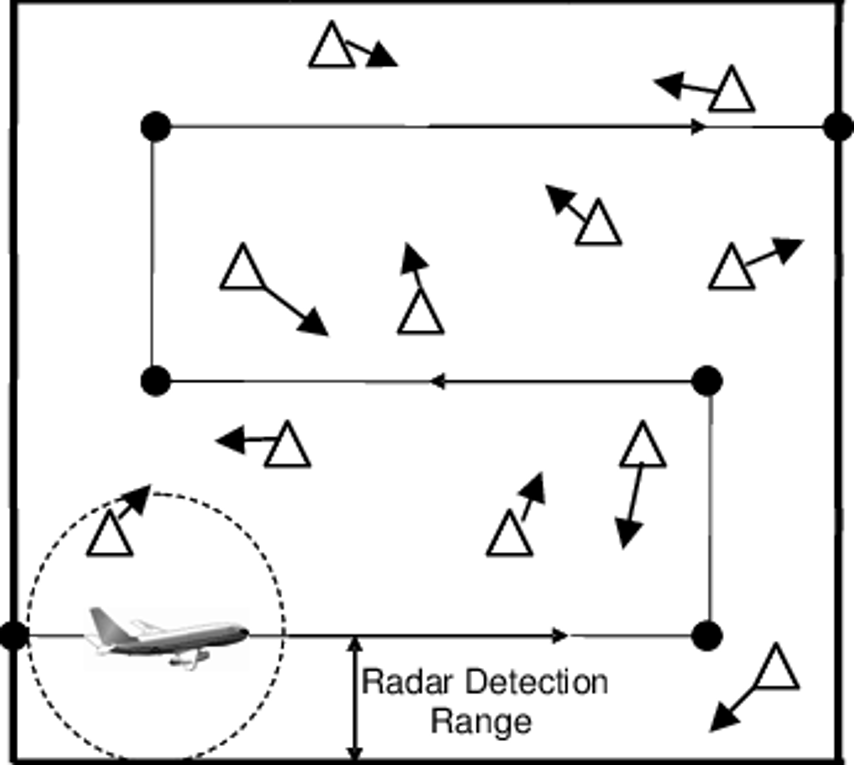
\includegraphics[width=\linewidth]{fig/vant.png}
        \column{0.5\textwidth}
        \centering
        \begin{itemize}
            \item Utilizar \textit{simulated annealing} para resolver o TSP com “cidades” surgindo ao longo da missão
            \item Cada novo alvo detectado torna-se um vértice candidato
            \item A decisão de inserção considera a distância entre o alvo e a rota atual
            \item Se estiver dentro do limite, o vértice é aceito e a rota é recalculada com \textit{simulated annealing}
        \end{itemize}
    \end{columns}
\end{frame}

\begin{frame}{Simplificações}
    \begin{columns}
        \column{0.5\textwidth}
        \centering
        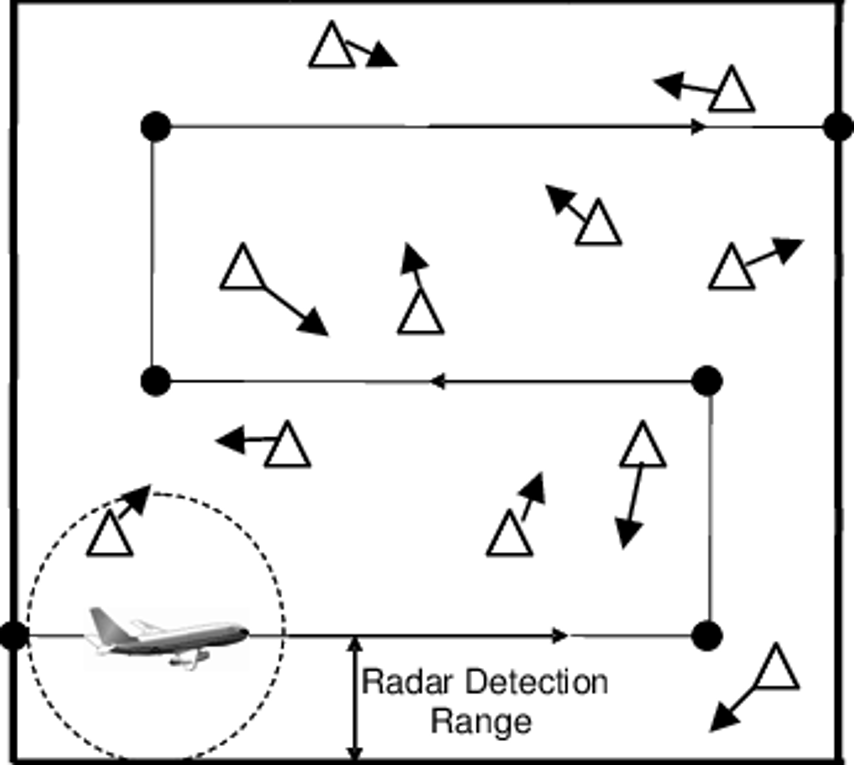
\includegraphics[width=\linewidth]{fig/vant.png}
        \column{0.5\textwidth}
        \centering
        \begin{itemize}
            \item Navios são considerados estáticos (em relação ao VANT)
            \item A dinâmica da aeronave é desprezada na modelagem
        \end{itemize}
    \end{columns}
\end{frame}

\begin{frame}{Obrigado!}
\centering
\Large Dúvidas?
\end{frame}

%--------------------------------------------------------------
% \section{Referências}

% \begin{frame}{Referências}
%     Exemplo de citação: \cite{placeholder}.
    
%     \bibliographystyle{plain}
%     \bibliography{referencias}
% \end{frame}

\end{document}
